% Options for packages loaded elsewhere
\PassOptionsToPackage{unicode}{hyperref}
\PassOptionsToPackage{hyphens}{url}
%
\documentclass[
]{article}
\usepackage{lmodern}
\usepackage{amssymb,amsmath}
\usepackage{ifxetex,ifluatex}
\ifnum 0\ifxetex 1\fi\ifluatex 1\fi=0 % if pdftex
  \usepackage[T1]{fontenc}
  \usepackage[utf8]{inputenc}
  \usepackage{textcomp} % provide euro and other symbols
\else % if luatex or xetex
  \usepackage{unicode-math}
  \defaultfontfeatures{Scale=MatchLowercase}
  \defaultfontfeatures[\rmfamily]{Ligatures=TeX,Scale=1}
\fi
% Use upquote if available, for straight quotes in verbatim environments
\IfFileExists{upquote.sty}{\usepackage{upquote}}{}
\IfFileExists{microtype.sty}{% use microtype if available
  \usepackage[]{microtype}
  \UseMicrotypeSet[protrusion]{basicmath} % disable protrusion for tt fonts
}{}
\makeatletter
\@ifundefined{KOMAClassName}{% if non-KOMA class
  \IfFileExists{parskip.sty}{%
    \usepackage{parskip}
  }{% else
    \setlength{\parindent}{0pt}
    \setlength{\parskip}{6pt plus 2pt minus 1pt}}
}{% if KOMA class
  \KOMAoptions{parskip=half}}
\makeatother
\usepackage{xcolor}
\IfFileExists{xurl.sty}{\usepackage{xurl}}{} % add URL line breaks if available
\IfFileExists{bookmark.sty}{\usepackage{bookmark}}{\usepackage{hyperref}}
\hypersetup{
  pdftitle={Data Manipulation},
  hidelinks,
  pdfcreator={LaTeX via pandoc}}
\urlstyle{same} % disable monospaced font for URLs
\usepackage[margin=1in]{geometry}
\usepackage{color}
\usepackage{fancyvrb}
\newcommand{\VerbBar}{|}
\newcommand{\VERB}{\Verb[commandchars=\\\{\}]}
\DefineVerbatimEnvironment{Highlighting}{Verbatim}{commandchars=\\\{\}}
% Add ',fontsize=\small' for more characters per line
\usepackage{framed}
\definecolor{shadecolor}{RGB}{248,248,248}
\newenvironment{Shaded}{\begin{snugshade}}{\end{snugshade}}
\newcommand{\AlertTok}[1]{\textcolor[rgb]{0.94,0.16,0.16}{#1}}
\newcommand{\AnnotationTok}[1]{\textcolor[rgb]{0.56,0.35,0.01}{\textbf{\textit{#1}}}}
\newcommand{\AttributeTok}[1]{\textcolor[rgb]{0.77,0.63,0.00}{#1}}
\newcommand{\BaseNTok}[1]{\textcolor[rgb]{0.00,0.00,0.81}{#1}}
\newcommand{\BuiltInTok}[1]{#1}
\newcommand{\CharTok}[1]{\textcolor[rgb]{0.31,0.60,0.02}{#1}}
\newcommand{\CommentTok}[1]{\textcolor[rgb]{0.56,0.35,0.01}{\textit{#1}}}
\newcommand{\CommentVarTok}[1]{\textcolor[rgb]{0.56,0.35,0.01}{\textbf{\textit{#1}}}}
\newcommand{\ConstantTok}[1]{\textcolor[rgb]{0.00,0.00,0.00}{#1}}
\newcommand{\ControlFlowTok}[1]{\textcolor[rgb]{0.13,0.29,0.53}{\textbf{#1}}}
\newcommand{\DataTypeTok}[1]{\textcolor[rgb]{0.13,0.29,0.53}{#1}}
\newcommand{\DecValTok}[1]{\textcolor[rgb]{0.00,0.00,0.81}{#1}}
\newcommand{\DocumentationTok}[1]{\textcolor[rgb]{0.56,0.35,0.01}{\textbf{\textit{#1}}}}
\newcommand{\ErrorTok}[1]{\textcolor[rgb]{0.64,0.00,0.00}{\textbf{#1}}}
\newcommand{\ExtensionTok}[1]{#1}
\newcommand{\FloatTok}[1]{\textcolor[rgb]{0.00,0.00,0.81}{#1}}
\newcommand{\FunctionTok}[1]{\textcolor[rgb]{0.00,0.00,0.00}{#1}}
\newcommand{\ImportTok}[1]{#1}
\newcommand{\InformationTok}[1]{\textcolor[rgb]{0.56,0.35,0.01}{\textbf{\textit{#1}}}}
\newcommand{\KeywordTok}[1]{\textcolor[rgb]{0.13,0.29,0.53}{\textbf{#1}}}
\newcommand{\NormalTok}[1]{#1}
\newcommand{\OperatorTok}[1]{\textcolor[rgb]{0.81,0.36,0.00}{\textbf{#1}}}
\newcommand{\OtherTok}[1]{\textcolor[rgb]{0.56,0.35,0.01}{#1}}
\newcommand{\PreprocessorTok}[1]{\textcolor[rgb]{0.56,0.35,0.01}{\textit{#1}}}
\newcommand{\RegionMarkerTok}[1]{#1}
\newcommand{\SpecialCharTok}[1]{\textcolor[rgb]{0.00,0.00,0.00}{#1}}
\newcommand{\SpecialStringTok}[1]{\textcolor[rgb]{0.31,0.60,0.02}{#1}}
\newcommand{\StringTok}[1]{\textcolor[rgb]{0.31,0.60,0.02}{#1}}
\newcommand{\VariableTok}[1]{\textcolor[rgb]{0.00,0.00,0.00}{#1}}
\newcommand{\VerbatimStringTok}[1]{\textcolor[rgb]{0.31,0.60,0.02}{#1}}
\newcommand{\WarningTok}[1]{\textcolor[rgb]{0.56,0.35,0.01}{\textbf{\textit{#1}}}}
\usepackage{graphicx}
\makeatletter
\def\maxwidth{\ifdim\Gin@nat@width>\linewidth\linewidth\else\Gin@nat@width\fi}
\def\maxheight{\ifdim\Gin@nat@height>\textheight\textheight\else\Gin@nat@height\fi}
\makeatother
% Scale images if necessary, so that they will not overflow the page
% margins by default, and it is still possible to overwrite the defaults
% using explicit options in \includegraphics[width, height, ...]{}
\setkeys{Gin}{width=\maxwidth,height=\maxheight,keepaspectratio}
% Set default figure placement to htbp
\makeatletter
\def\fps@figure{htbp}
\makeatother
\setlength{\emergencystretch}{3em} % prevent overfull lines
\providecommand{\tightlist}{%
  \setlength{\itemsep}{0pt}\setlength{\parskip}{0pt}}
\setcounter{secnumdepth}{-\maxdimen} % remove section numbering

\title{Data Manipulation}
\author{}
\date{\vspace{-2.5em}}

\begin{document}
\maketitle

\hypertarget{practical-03}{%
\section{Practical 03}\label{practical-03}}

\hypertarget{preamble}{%
\subsection{Preamble}\label{preamble}}

\begin{Shaded}
\begin{Highlighting}[]
\CommentTok{\#\# (01) Clean up the Iris Data}

\CommentTok{\# Preamble}
\CommentTok{\#\# Install Pacman}
\NormalTok{load.pac <{-}}\StringTok{ }\ControlFlowTok{function}\NormalTok{() \{}
  
  \ControlFlowTok{if}\NormalTok{(}\KeywordTok{require}\NormalTok{(}\StringTok{"pacman"}\NormalTok{))\{}
    \KeywordTok{library}\NormalTok{(pacman)}
\NormalTok{  \}}\ControlFlowTok{else}\NormalTok{\{}
    \KeywordTok{install.packages}\NormalTok{(}\StringTok{"pacman"}\NormalTok{)}
    \KeywordTok{library}\NormalTok{(pacman)}
\NormalTok{  \}}
  
\NormalTok{  pacman}\OperatorTok{::}\KeywordTok{p\_load}\NormalTok{(xts, sp, gstat, ggplot2, rmarkdown, reshape2, ggmap,}
\NormalTok{                 parallel, dplyr, plotly, tidyverse, reticulate, UsingR, Rmpfr,}
\NormalTok{                 swirl, corrplot, gridExtra, mise, latex2exp, tree, rpart)}
  
\NormalTok{\}}

\KeywordTok{load.pac}\NormalTok{()}
\end{Highlighting}
\end{Shaded}

\begin{verbatim}
## Loading required package: pacman
\end{verbatim}

\begin{Shaded}
\begin{Highlighting}[]
\KeywordTok{mise}\NormalTok{()}
\end{Highlighting}
\end{Shaded}

\newpage{}

\hypertarget{reading-in-iris-data}{%
\subsection{(01) Reading in iris data}\label{reading-in-iris-data}}

\begin{Shaded}
\begin{Highlighting}[]
\NormalTok{iris\_bad <{-}}\StringTok{ }\KeywordTok{read.csv}\NormalTok{(}\DataTypeTok{file =} \StringTok{"./DataSets/iris\_badvalues.csv"}\NormalTok{, }\DataTypeTok{header =} \OtherTok{TRUE}\NormalTok{, }\DataTypeTok{sep =} \StringTok{","}\NormalTok{)}
\KeywordTok{load}\NormalTok{(}\DataTypeTok{file =} \StringTok{"./iriswithbadvalues.RData"}\NormalTok{)}

\KeywordTok{head}\NormalTok{(iris\_bad)}
\end{Highlighting}
\end{Shaded}

\begin{verbatim}
##   Sample.Index Sepal.Length Sepal.Width Petal.Length Petal.Width Species
## 1            1          5.1         3.5          1.4         0.2  setosa
## 2            2          4.9         3.0          1.4         0.2  setosa
## 3            3          4.7         3.2          1.3         0.2  setosa
## 4            4          4.6         3.1         -1.0         0.2  setosa
## 5            5          5.0          NA          1.4         0.2  setosa
## 6            6          5.4         3.9          1.7          NA  setosa
\end{verbatim}

\begin{Shaded}
\begin{Highlighting}[]
\KeywordTok{str}\NormalTok{(iris\_bad)}
\end{Highlighting}
\end{Shaded}

\begin{verbatim}
## 'data.frame':    150 obs. of  6 variables:
##  $ Sample.Index: int  1 2 3 4 5 6 7 8 9 10 ...
##  $ Sepal.Length: num  5.1 4.9 4.7 4.6 5 5.4 4.6 5 4.4 4.9 ...
##  $ Sepal.Width : num  3.5 3 3.2 3.1 NA 3.9 3.4 3.4 2.9 3.1 ...
##  $ Petal.Length: num  1.4 1.4 1.3 -1 1.4 1.7 NA 1.5 1.4 1.5 ...
##  $ Petal.Width : num  0.2 0.2 0.2 0.2 0.2 NA 0.3 0.2 0.2 0.1 ...
##  $ Species     : Factor w/ 3 levels "setosa","versicolor",..: 1 1 1 1 1 1 1 1 1 1 ...
\end{verbatim}

\begin{Shaded}
\begin{Highlighting}[]
\KeywordTok{summary}\NormalTok{(iris\_bad)}
\end{Highlighting}
\end{Shaded}

\begin{verbatim}
##   Sample.Index     Sepal.Length     Sepal.Width    Petal.Length   
##  Min.   :  1.00   Min.   :-5.700   Min.   :0.00   Min.   :-6.000  
##  1st Qu.: 38.25   1st Qu.: 5.100   1st Qu.:2.80   1st Qu.: 1.600  
##  Median : 75.50   Median : 5.800   Median :3.00   Median : 4.350  
##  Mean   : 75.50   Mean   : 5.724   Mean   :3.01   Mean   : 3.703  
##  3rd Qu.:112.75   3rd Qu.: 6.400   3rd Qu.:3.30   3rd Qu.: 5.100  
##  Max.   :150.00   Max.   : 7.900   Max.   :4.40   Max.   : 6.900  
##                   NA's   :10       NA's   :12     NA's   :12      
##   Petal.Width          Species  
##  Min.   :0.000   setosa    :50  
##  1st Qu.:0.300   versicolor:50  
##  Median :1.300   virginica :50  
##  Mean   :1.203                  
##  3rd Qu.:1.800                  
##  Max.   :2.500                  
##  NA's   :1
\end{verbatim}

\hypertarget{clean-the-data}{%
\subsubsection{Clean the Data}\label{clean-the-data}}

Copy the data into another data frame to work with:

\begin{Shaded}
\begin{Highlighting}[]
\NormalTok{(iris\_tib <{-}}\StringTok{ }\KeywordTok{as\_tibble}\NormalTok{(iris\_bad))}
\end{Highlighting}
\end{Shaded}

\begin{verbatim}
## # A tibble: 150 x 6
##    Sample.Index Sepal.Length Sepal.Width Petal.Length Petal.Width Species
##           <int>        <dbl>       <dbl>        <dbl>       <dbl> <fct>  
##  1            1          5.1         3.5          1.4         0.2 setosa 
##  2            2          4.9         3            1.4         0.2 setosa 
##  3            3          4.7         3.2          1.3         0.2 setosa 
##  4            4          4.6         3.1         -1           0.2 setosa 
##  5            5          5          NA            1.4         0.2 setosa 
##  6            6          5.4         3.9          1.7        NA   setosa 
##  7            7          4.6         3.4         NA           0.3 setosa 
##  8            8          5           3.4          1.5         0.2 setosa 
##  9            9          4.4         2.9          1.4         0.2 setosa 
## 10           10          4.9         3.1          1.5         0.1 setosa 
## # ... with 140 more rows
\end{verbatim}

\begin{Shaded}
\begin{Highlighting}[]
\NormalTok{iris\_df <{-}}\StringTok{ }\NormalTok{iris\_bad}
\end{Highlighting}
\end{Shaded}

\hypertarget{negative-values}{%
\paragraph{Negative Values}\label{negative-values}}

\hypertarget{remove-negative-values}{%
\subparagraph{Remove Negative Values}\label{remove-negative-values}}

In order to remove negative values the \texttt{abs} function could be
used:

\begin{Shaded}
\begin{Highlighting}[]
\CommentTok{\# Easy Built in}
\NormalTok{iris\_df[, }\DecValTok{1}\OperatorTok{:}\DecValTok{5}\NormalTok{] }\OperatorTok{\%>\%}\StringTok{ }\KeywordTok{abs}\NormalTok{() }\OperatorTok{\%>\%}\StringTok{ }\KeywordTok{head}\NormalTok{()}
\end{Highlighting}
\end{Shaded}

\begin{verbatim}
##   Sample.Index Sepal.Length Sepal.Width Petal.Length Petal.Width
## 1            1          5.1         3.5          1.4         0.2
## 2            2          4.9         3.0          1.4         0.2
## 3            3          4.7         3.2          1.3         0.2
## 4            4          4.6         3.1          1.0         0.2
## 5            5          5.0          NA          1.4         0.2
## 6            6          5.4         3.9          1.7          NA
\end{verbatim}

\begin{Shaded}
\begin{Highlighting}[]
\NormalTok{iris\_tib[, }\DecValTok{1}\OperatorTok{:}\DecValTok{5}\NormalTok{] }\OperatorTok{\%>\%}\StringTok{ }\KeywordTok{abs}\NormalTok{() }\OperatorTok{\%>\%}\StringTok{ }\KeywordTok{head}\NormalTok{()}
\end{Highlighting}
\end{Shaded}

\begin{verbatim}
## # A tibble: 6 x 5
##   Sample.Index Sepal.Length Sepal.Width Petal.Length Petal.Width
##          <int>        <dbl>       <dbl>        <dbl>       <dbl>
## 1            1          5.1         3.5          1.4         0.2
## 2            2          4.9         3            1.4         0.2
## 3            3          4.7         3.2          1.3         0.2
## 4            4          4.6         3.1          1           0.2
## 5            5          5          NA            1.4         0.2
## 6            6          5.4         3.9          1.7        NA
\end{verbatim}

It's always possible to roll your own function but in doing so it is
necessary to:

\begin{enumerate}
\def\labelenumi{\arabic{enumi}.}
\tightlist
\item
  Check for \texttt{na} values
\end{enumerate}

\begin{itemize}
\tightlist
\item
  notice that \texttt{is.numeric()} will return \texttt{TRUE} if the
  \texttt{NA} value is an element of a \texttt{data.frame}, for this
  reason use \texttt{!\ is.na()}
\end{itemize}

\begin{enumerate}
\def\labelenumi{\arabic{enumi}.}
\setcounter{enumi}{1}
\tightlist
\item
  Don't assign Null Values
\end{enumerate}

So it's usually better to use built in functions where possible:

\begin{Shaded}
\begin{Highlighting}[]
\CommentTok{\# Roll your own}

\NormalTok{my\_abs <{-}}\StringTok{ }\ControlFlowTok{function}\NormalTok{(x) \{}
  \ControlFlowTok{if}\NormalTok{ (}\OperatorTok{!}\KeywordTok{is.na}\NormalTok{(x)) \{}
    \ControlFlowTok{if}\NormalTok{ (x }\OperatorTok{<}\StringTok{ }\DecValTok{0}\NormalTok{) \{}
      \OperatorTok{{-}}\NormalTok{x}
\NormalTok{    \} }\ControlFlowTok{else}\NormalTok{ \{}
\NormalTok{      x}
\NormalTok{    \}}
\NormalTok{  \}}
\NormalTok{\}}


\NormalTok{new\_df <{-}}\StringTok{ }\NormalTok{iris\_df}
\ControlFlowTok{for}\NormalTok{ (r }\ControlFlowTok{in} \DecValTok{1}\OperatorTok{:}\KeywordTok{nrow}\NormalTok{(iris\_df)) \{}
  \ControlFlowTok{for}\NormalTok{ (c }\ControlFlowTok{in} \DecValTok{1}\OperatorTok{:}\DecValTok{5}\NormalTok{) \{}
    \ControlFlowTok{if}\NormalTok{ (}\KeywordTok{length}\NormalTok{(}\KeywordTok{my\_abs}\NormalTok{(iris\_df[r, c])) }\OperatorTok{==}\StringTok{ }\DecValTok{1}\NormalTok{) \{}
\NormalTok{      new\_df[r, c] <{-}}\StringTok{ }\KeywordTok{my\_abs}\NormalTok{(iris\_df[r, c])}
\NormalTok{    \}}
\NormalTok{  \}}
\NormalTok{\}}
\NormalTok{new\_df }\OperatorTok{\%>\%}\StringTok{ }\KeywordTok{head}\NormalTok{()}
\end{Highlighting}
\end{Shaded}

\begin{verbatim}
##   Sample.Index Sepal.Length Sepal.Width Petal.Length Petal.Width Species
## 1            1          5.1         3.5          1.4         0.2  setosa
## 2            2          4.9         3.0          1.4         0.2  setosa
## 3            3          4.7         3.2          1.3         0.2  setosa
## 4            4          4.6         3.1          1.0         0.2  setosa
## 5            5          5.0          NA          1.4         0.2  setosa
## 6            6          5.4         3.9          1.7          NA  setosa
\end{verbatim}

\hypertarget{show-negative-values}{%
\subparagraph{Show Negative Values}\label{show-negative-values}}

Base Packages

We may wan't to preview rows that have negative values rather than just
making them positive.

A possible way to do this is to use \texttt{df{[}df\textless{}0{]}}, but
tht will not work with tibbles, instead create a logical matrix in order
to find the negative values, bear in mind that \textbf{\emph{R}}
consideres any number that isn't 0 to be \emph{truthy} so \texttt{sum()}
and \texttt{prod()} may be used to with \texttt{apply()} to create
logical tests:

\begin{verbatim}
| Description | Command   | Code Syntax | Mathematical |
| ---         | ----      | --          | ---          |
| And         | `prod()` / $\Pi^n_{i=1}$ | `&`   | $\wedge$     |
| Or          | `sum` / $\sum^n_{i=1}$ | `|`     | $\vee$       |
\end{verbatim}

This method will work with both tibbles and data frames.

\begin{Shaded}
\begin{Highlighting}[]
\CommentTok{\# is the entry negative but not missing}
\NormalTok{is\_neg <{-}}\StringTok{ }\NormalTok{iris\_df[,}\DecValTok{1}\OperatorTok{:}\DecValTok{5}\NormalTok{]}\OperatorTok{<}\DecValTok{0} \OperatorTok{\&}\StringTok{ }\OperatorTok{!}\KeywordTok{is.na}\NormalTok{(iris\_df[,}\DecValTok{1}\OperatorTok{:}\DecValTok{5}\NormalTok{]) }
\CommentTok{\# is any column in the row negative?}
  \CommentTok{\# **and** / $\^{}$ ; is \textasciigrave{}prod()\textasciigrave{}, **or** / $V$ is \textasciigrave{}sum()\textasciigrave{}}
\NormalTok{is\_row\_neg <{-}}\StringTok{ }\KeywordTok{apply}\NormalTok{(is\_neg, }\DecValTok{1}\NormalTok{, sum) }\OperatorTok{\%>\%}\StringTok{ }\KeywordTok{as.logical}\NormalTok{()}
\CommentTok{\# Which Rows are negatives}
\NormalTok{neg\_rows <{-}}\StringTok{ }\KeywordTok{which}\NormalTok{(is\_row\_neg)}

\CommentTok{\# Return the rows that contain negative observations}
\NormalTok{negvals  <{-}}\StringTok{ }\NormalTok{iris\_df[neg\_rows,]}
\NormalTok{meanvals <{-}}\StringTok{ }\KeywordTok{apply}\NormalTok{(}\KeywordTok{na.omit}\NormalTok{(}\KeywordTok{abs}\NormalTok{(iris\_df[,}\OperatorTok{{-}}\DecValTok{6}\NormalTok{])), }\DecValTok{2}\NormalTok{, mean) }\OperatorTok{\%>\%}\StringTok{ }\KeywordTok{round}\NormalTok{(}\DecValTok{1}\NormalTok{)}
\NormalTok{sdvals   <{-}}\StringTok{ }\KeywordTok{apply}\NormalTok{(}\KeywordTok{na.omit}\NormalTok{(}\KeywordTok{abs}\NormalTok{(iris\_df[,}\OperatorTok{{-}}\DecValTok{6}\NormalTok{])), }\DecValTok{2}\NormalTok{, sd) }\OperatorTok{\%>\%}\StringTok{ }\KeywordTok{round}\NormalTok{(}\DecValTok{2}\NormalTok{)}
\KeywordTok{rbind}\NormalTok{(negvals, meanvals, sdvals) }
\end{Highlighting}
\end{Shaded}

\begin{verbatim}
## Warning in `[<-.factor`(`*tmp*`, ri, value = 78): invalid factor level, NA
## generated

## Warning in `[<-.factor`(`*tmp*`, ri, value = 78): invalid factor level, NA
## generated
\end{verbatim}

\begin{verbatim}
##     Sample.Index Sepal.Length Sepal.Width Petal.Length Petal.Width   Species
## 4           4.00         4.60        3.10        -1.00        0.20    setosa
## 19         19.00        -5.70          NA         1.70        0.30    setosa
## 101       101.00         6.30        3.30        -6.00        2.50 virginica
## 41         78.00         5.80        3.00         3.80        1.20      <NA>
## 5          42.45         0.85        0.49         1.76        0.75      <NA>
\end{verbatim}

\begin{Shaded}
\begin{Highlighting}[]
\CommentTok{\# Remove Rows that have negative values}
\CommentTok{\# iris\_df[{-}neg\_rows,]}
\end{Highlighting}
\end{Shaded}

TidyVerse

In order to view negative values with tibbles it's quite simple to use
\texttt{dplyr}:

\begin{Shaded}
\begin{Highlighting}[]
\NormalTok{iris\_tib }\OperatorTok{\%>\%}
\StringTok{  }\NormalTok{dplyr}\OperatorTok{::}\KeywordTok{filter}\NormalTok{(Petal.Length }\OperatorTok{<}\StringTok{ }\DecValTok{0} \OperatorTok{|}\StringTok{  }\NormalTok{Sepal.Length }\OperatorTok{<}\StringTok{ }\DecValTok{0} \OperatorTok{|}\StringTok{  }\NormalTok{Petal.Width}\OperatorTok{<}\StringTok{ }\DecValTok{0} \OperatorTok{|}\StringTok{  }\NormalTok{Sepal.Width}\OperatorTok{<}\StringTok{ }\DecValTok{0}\NormalTok{ )}
\end{Highlighting}
\end{Shaded}

\begin{verbatim}
## # A tibble: 3 x 6
##   Sample.Index Sepal.Length Sepal.Width Petal.Length Petal.Width Species  
##          <int>        <dbl>       <dbl>        <dbl>       <dbl> <fct>    
## 1            4          4.6         3.1         -1           0.2 setosa   
## 2           19         -5.7        NA            1.7         0.3 setosa   
## 3          101          6.3         3.3         -6           2.5 virginica
\end{verbatim}

if you don't want to type in all the column names it might be ideal to
transform the table into \texttt{longer} format \textgreater{} (like
tidy data but more about making it longer so there's only one relevant
column not necessarily conforming to the rules of tidy)

\begin{Shaded}
\begin{Highlighting}[]
\CommentTok{\# Make it Longer}

\KeywordTok{pivot\_longer}\NormalTok{(iris\_tib, }\DataTypeTok{cols =} \KeywordTok{names}\NormalTok{(iris\_df)[}\DecValTok{2}\OperatorTok{:}\DecValTok{5}\NormalTok{]) }
\end{Highlighting}
\end{Shaded}

\begin{verbatim}
## # A tibble: 600 x 4
##    Sample.Index Species name         value
##           <int> <fct>   <chr>        <dbl>
##  1            1 setosa  Sepal.Length   5.1
##  2            1 setosa  Sepal.Width    3.5
##  3            1 setosa  Petal.Length   1.4
##  4            1 setosa  Petal.Width    0.2
##  5            2 setosa  Sepal.Length   4.9
##  6            2 setosa  Sepal.Width    3  
##  7            2 setosa  Petal.Length   1.4
##  8            2 setosa  Petal.Width    0.2
##  9            3 setosa  Sepal.Length   4.7
## 10            3 setosa  Sepal.Width    3.2
## # ... with 590 more rows
\end{verbatim}

\begin{Shaded}
\begin{Highlighting}[]
\CommentTok{\# Filter out Negative Results}
\KeywordTok{pivot\_longer}\NormalTok{(iris\_tib, }\DataTypeTok{cols =} \KeywordTok{names}\NormalTok{(iris\_df)[}\DecValTok{2}\OperatorTok{:}\DecValTok{5}\NormalTok{]) }\OperatorTok{\%>\%}\StringTok{ }
\StringTok{  }\NormalTok{dplyr}\OperatorTok{::}\KeywordTok{filter}\NormalTok{(value }\OperatorTok{<}\StringTok{ }\DecValTok{0}\NormalTok{) }
\end{Highlighting}
\end{Shaded}

\begin{verbatim}
## # A tibble: 3 x 4
##   Sample.Index Species   name         value
##          <int> <fct>     <chr>        <dbl>
## 1            4 setosa    Petal.Length  -1  
## 2           19 setosa    Sepal.Length  -5.7
## 3          101 virginica Petal.Length  -6
\end{verbatim}

Discussing Negative Values

The negative values seem to be pretty close to what was expected so they
won't be removed but converted to positive values.

\begin{Shaded}
\begin{Highlighting}[]
\NormalTok{iris\_df[,}\OperatorTok{{-}}\DecValTok{6}\NormalTok{] <{-}}\StringTok{ }\KeywordTok{abs}\NormalTok{(iris\_df[,}\OperatorTok{{-}}\DecValTok{6}\NormalTok{])}
\NormalTok{iris\_tib[,}\OperatorTok{{-}}\DecValTok{6}\NormalTok{] <{-}}\StringTok{ }\KeywordTok{abs}\NormalTok{(iris\_tib[,}\OperatorTok{{-}}\DecValTok{6}\NormalTok{])}
\end{Highlighting}
\end{Shaded}

\hypertarget{zero-values}{%
\paragraph{Zero Values}\label{zero-values}}

Before values that are too large can be considered, it is necessary to
remove the zero values.

the zero values can be removed for a data frame or matrix by using
na.omit (this doesn't work for tibbles):

\begin{Shaded}
\begin{Highlighting}[]
\NormalTok{iris\_df[iris\_df}\OperatorTok{==}\DecValTok{0}\NormalTok{] <{-}}\StringTok{ }\OtherTok{NA}
\KeywordTok{na.omit}\NormalTok{(iris\_df) }\OperatorTok{\%>\%}\StringTok{ }\KeywordTok{head}\NormalTok{()}
\end{Highlighting}
\end{Shaded}

\begin{verbatim}
##   Sample.Index Sepal.Length Sepal.Width Petal.Length Petal.Width Species
## 1            1          5.1         3.5          1.4         0.2  setosa
## 2            2          4.9         3.0          1.4         0.2  setosa
## 3            3          4.7         3.2          1.3         0.2  setosa
## 4            4          4.6         3.1          1.0         0.2  setosa
## 8            8          5.0         3.4          1.5         0.2  setosa
## 9            9          4.4         2.9          1.4         0.2  setosa
\end{verbatim}

\hypertarget{view-zero-observations}{%
\subparagraph{View Zero Observations}\label{view-zero-observations}}

The observations with zeroes can be previewed:

\begin{Shaded}
\begin{Highlighting}[]
\NormalTok{is\_zero <{-}iris\_tib}\OperatorTok{==}\DecValTok{0}
\NormalTok{is\_zero[}\KeywordTok{is.na}\NormalTok{(is\_zero)] <{-}}\StringTok{ }\OtherTok{FALSE}
\NormalTok{zero\_rows <{-}}\StringTok{ }\KeywordTok{apply}\NormalTok{(is\_zero, }\DecValTok{1}\NormalTok{, sum) }\OperatorTok{\%>\%}\StringTok{ }\KeywordTok{as.logical}\NormalTok{()}

\NormalTok{iris\_tib[zero\_rows,] }\OperatorTok{\%>\%}\StringTok{ }\KeywordTok{head}\NormalTok{()}
\end{Highlighting}
\end{Shaded}

\begin{verbatim}
## # A tibble: 4 x 6
##   Sample.Index Sepal.Length Sepal.Width Petal.Length Petal.Width Species   
##          <int>        <dbl>       <dbl>        <dbl>       <dbl> <fct>     
## 1           12         NA           3.4          1.6         0   setosa    
## 2           84          6           0           NA           1.6 versicolor
## 3          117          6.5         0            5.5         1.8 virginica 
## 4          142          0          NA            5.1         2.3 virginica
\end{verbatim}

in order to remove these values use the following:

\begin{Shaded}
\begin{Highlighting}[]
\NormalTok{iris\_tib[}\OperatorTok{{-}}\NormalTok{zero\_rows, ] }\OperatorTok{\%>\%}\StringTok{ }\KeywordTok{head}\NormalTok{()}
\end{Highlighting}
\end{Shaded}

\begin{verbatim}
## # A tibble: 6 x 6
##   Sample.Index Sepal.Length Sepal.Width Petal.Length Petal.Width Species
##          <int>        <dbl>       <dbl>        <dbl>       <dbl> <fct>  
## 1            2          4.9         3            1.4         0.2 setosa 
## 2            3          4.7         3.2          1.3         0.2 setosa 
## 3            4          4.6         3.1          1           0.2 setosa 
## 4            5          5          NA            1.4         0.2 setosa 
## 5            6          5.4         3.9          1.7        NA   setosa 
## 6            7          4.6         3.4         NA           0.3 setosa
\end{verbatim}

\hypertarget{values-that-are-too-large}{%
\paragraph{Values that are too Large}\label{values-that-are-too-large}}

In order to consider values that are too large the mean value and
standard deviation can be used.

Create a function to return the index values of a vector which has
values that are extremely far from the mean.

\begin{itemize}
\tightlist
\item
  Create an argument to specify the probability of detecting an extreme
  value assuming that value is to be expected from the population

  \begin{itemize}
  \tightlist
  \item
    This would be the \(\alpha\) level / the FPR / the probability of a
    type I error.
  \end{itemize}
\end{itemize}

\begin{Shaded}
\begin{Highlighting}[]
\CommentTok{\# This Function will take a vector as input and a False Positive Rate}
    \CommentTok{\# It will return the index values that are sufficiently far from the }
    \CommentTok{\# the mean to indicate that they are extreme (considering the variance)}
        \CommentTok{\# Assuming there is no difference, the probability detecting one}
        \CommentTok{\# is the FPR}

\NormalTok{is\_extreme <{-}}\StringTok{ }\ControlFlowTok{function}\NormalTok{(x, }\DataTypeTok{fpr=}\DecValTok{1}\OperatorTok{/}\DecValTok{100}\NormalTok{) \{}
\NormalTok{ Z   <{-}}\StringTok{ }\KeywordTok{abs}\NormalTok{(}\KeywordTok{qnorm}\NormalTok{(fpr}\OperatorTok{/}\DecValTok{2}\NormalTok{, }\DecValTok{0}\NormalTok{, }\DecValTok{1}\NormalTok{)) }
\NormalTok{ mu  <{-}}\StringTok{ }\KeywordTok{mean}\NormalTok{(}\KeywordTok{na.omit}\NormalTok{(x))}
\NormalTok{ sig <{-}}\StringTok{ }\KeywordTok{sd}\NormalTok{(}\KeywordTok{na.omit}\NormalTok{(x)) }
  
\NormalTok{  is\_small <{-}}\StringTok{ }\NormalTok{x }\OperatorTok{<}\StringTok{ }\NormalTok{mu }\OperatorTok{{-}}\StringTok{ }\NormalTok{Z }\OperatorTok{*}\StringTok{ }\NormalTok{sig}
\NormalTok{  is\_big   <{-}}\StringTok{ }\NormalTok{x }\OperatorTok{>}\StringTok{ }\NormalTok{mu }\OperatorTok{+}\StringTok{ }\NormalTok{Z }\OperatorTok{*}\StringTok{ }\NormalTok{sig}
  
\NormalTok{  is\_small }\OperatorTok{|}\StringTok{ }\NormalTok{is\_big}
\NormalTok{\}}

\NormalTok{extreme\_vals <{-}}\StringTok{ }\ControlFlowTok{function}\NormalTok{(x, fpr) \{}
 \KeywordTok{which}\NormalTok{(}\KeywordTok{is\_extreme}\NormalTok{(x, fpr)) }
\NormalTok{\}}

\CommentTok{\#   \# Example}
\CommentTok{\# rvals <{-} rnorm(100)}
\CommentTok{\# rvals[is\_extreme(rvals, fpr = 5/100)]}
\CommentTok{\# }
\CommentTok{\# \# Return Extreme Rows}
\CommentTok{\# iris\_df[,2] \%>\% extreme\_vals(fpr = 1/200)}
\CommentTok{\# iris\_df[,3] \%>\% extreme\_vals(fpr = 1/200)}
\CommentTok{\# iris\_df[,4] \%>\% extreme\_vals(fpr = 1/200)}
\CommentTok{\# iris\_df[,5] \%>\% extreme\_vals(fpr = 1/200)}

\NormalTok{extreme\_rows <{-}}\StringTok{ }\KeywordTok{c}\NormalTok{()}
\ControlFlowTok{for}\NormalTok{ (i }\ControlFlowTok{in} \DecValTok{2}\OperatorTok{:}\DecValTok{5}\NormalTok{) \{}
\NormalTok{  extreme\_rows <{-}}
\StringTok{    }\KeywordTok{c}\NormalTok{(extreme\_rows, }\KeywordTok{extreme\_vals}\NormalTok{(iris\_df[, i], }\DataTypeTok{fpr =} \DecValTok{1} \OperatorTok{/}\StringTok{ }\DecValTok{200}\NormalTok{))}
\NormalTok{\}}

\NormalTok{iris\_df[extreme\_rows,]}
\end{Highlighting}
\end{Shaded}

\begin{verbatim}
##    Sample.Index Sepal.Length Sepal.Width Petal.Length Petal.Width Species
## 16           16          5.7         4.4           NA         0.4  setosa
\end{verbatim}

Although this value is very far from the mean-value, it doesn't appear
to be any sort of transcription error, without good cause to remove the
data it will be left in.

\hypertarget{mis-spelling}{%
\paragraph{Mis-Spelling}\label{mis-spelling}}

Before this can be plotted it is necessary to make the \texttt{Species}
a factor, this will necessitate fixing mis-spellings.

Mis-Spellings can be checked by using \texttt{unique} and
\texttt{factor}:

\begin{Shaded}
\begin{Highlighting}[]
\KeywordTok{unique}\NormalTok{(iris\_df}\OperatorTok{$}\NormalTok{Species)}
\end{Highlighting}
\end{Shaded}

\begin{verbatim}
## [1] setosa     versicolor virginica 
## Levels: setosa versicolor virginica
\end{verbatim}

\hypertarget{duplicate-records}{%
\paragraph{Duplicate Records}\label{duplicate-records}}

Duplicate Records can be checked by using:

\begin{Shaded}
\begin{Highlighting}[]
\NormalTok{dupQ <{-}}\StringTok{ }\KeywordTok{duplicated}\NormalTok{(iris\_df)}
\NormalTok{iris\_df[dupQ,]}
\end{Highlighting}
\end{Shaded}

\begin{verbatim}
## [1] Sample.Index Sepal.Length Sepal.Width  Petal.Length Petal.Width 
## [6] Species     
## <0 rows> (or 0-length row.names)
\end{verbatim}

In this case no duplicate records could be identified.

\hypertarget{missing-values}{%
\paragraph{Missing Values}\label{missing-values}}

\hypertarget{should-values-be-removed}{%
\subparagraph{Should values be removed}\label{should-values-be-removed}}

Removing all missing records isn't necessarily desirable because the
missing element may be a feature that we are not concerned with
(e.g.~plotting sepal length and width but ignoring petal length), or it
may be appropriate to use some function to predict what that value could
be:

\begin{itemize}
\tightlist
\item
  using a Modelling Technique

  \begin{itemize}
  \tightlist
  \item
    Regression
  \item
    Classification Trees or random Forrest

    \begin{itemize}
    \tightlist
    \item
      Random Forrest
    \end{itemize}
  \end{itemize}
\item
  Using the mean Value
\item
  Using the median value
\end{itemize}

This can be particulary helpful if a dimension-reduction technique is
being used anyway.

For this reason this step will be performed

Modelling Missing Values

Trees are a really easy way to model missing values because there a type
of model that will \emph{tolerate} missing predictive variables, for
example to predict missing sepal length values:

\begin{Shaded}
\begin{Highlighting}[]
\NormalTok{iris\_df\_pred <{-}}\StringTok{ }\NormalTok{iris\_df}

\NormalTok{sep.tree <{-}}\StringTok{ }\KeywordTok{tree}\NormalTok{(}\DataTypeTok{formula =}\NormalTok{ Sepal.Length }\OperatorTok{\textasciitilde{}}\StringTok{ }\NormalTok{., }\DataTypeTok{data =} \KeywordTok{na.omit}\NormalTok{(iris\_df\_pred[,}\DecValTok{2}\OperatorTok{:}\DecValTok{5}\NormalTok{]))}

\KeywordTok{plot}\NormalTok{(sep.tree)}
\KeywordTok{text}\NormalTok{(sep.tree)}
\end{Highlighting}
\end{Shaded}

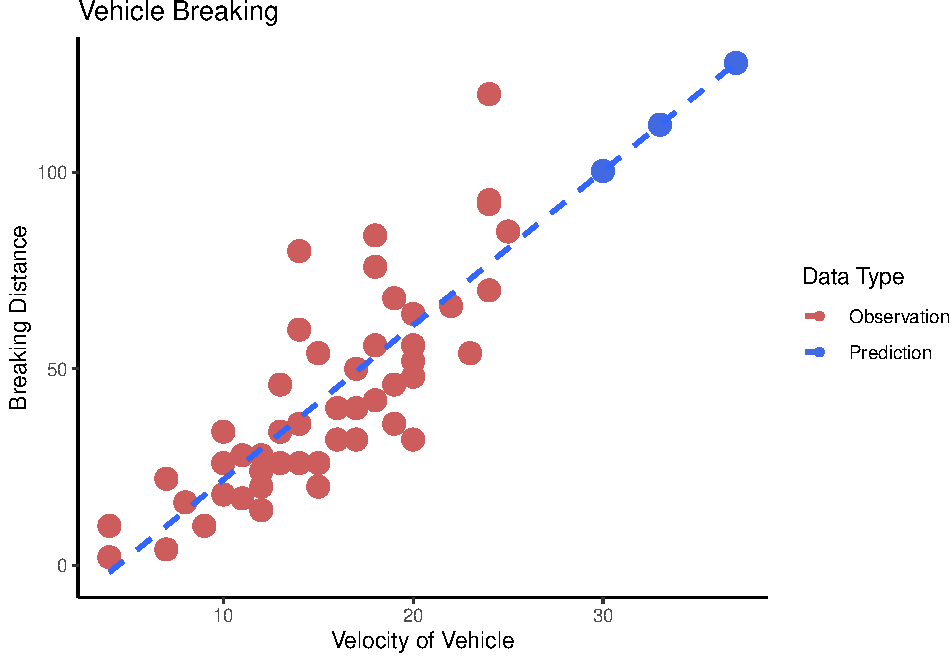
\includegraphics{03_vectors_files/figure-latex/unnamed-chunk-16-1.pdf}

\begin{Shaded}
\begin{Highlighting}[]
\NormalTok{missing\_sep\_length <{-}}\StringTok{ }\KeywordTok{which}\NormalTok{(}\KeywordTok{is.na}\NormalTok{(iris\_df\_pred}\OperatorTok{$}\NormalTok{Sepal.Length))}


\NormalTok{iris\_df\_pred[missing\_sep\_length,]}
\end{Highlighting}
\end{Shaded}

\begin{verbatim}
##     Sample.Index Sepal.Length Sepal.Width Petal.Length Petal.Width    Species
## 12            12           NA         3.4          1.6          NA     setosa
## 25            25           NA         3.4          1.9         0.2     setosa
## 31            31           NA         3.1          1.6         0.2     setosa
## 33            33           NA         4.1          1.5         0.1     setosa
## 37            37           NA         3.5           NA         0.2     setosa
## 59            59           NA         2.9          4.6         1.3 versicolor
## 93            93           NA          NA           NA         1.2 versicolor
## 114          114           NA         2.5          5.0         2.0  virginica
## 140          140           NA         3.1          5.4         2.1  virginica
## 142          142           NA          NA          5.1         2.3  virginica
## 144          144           NA         3.2          5.9         2.3  virginica
\end{verbatim}

\begin{Shaded}
\begin{Highlighting}[]
\NormalTok{iris\_df\_pred[missing\_sep\_length,}\DecValTok{2}\NormalTok{] <{-}}\StringTok{ }\KeywordTok{predict}\NormalTok{(sep.tree,}\DataTypeTok{newdata =}\NormalTok{ iris[missing\_sep\_length,])}
\NormalTok{iris\_df\_pred[missing\_sep\_length,]}
\end{Highlighting}
\end{Shaded}

\begin{verbatim}
##     Sample.Index Sepal.Length Sepal.Width Petal.Length Petal.Width    Species
## 12            12     5.160000         3.4          1.6          NA     setosa
## 25            25     5.160000         3.4          1.9         0.2     setosa
## 31            31     4.731579         3.1          1.6         0.2     setosa
## 33            33     5.160000         4.1          1.5         0.1     setosa
## 37            37     5.160000         3.5           NA         0.2     setosa
## 59            59     6.008333         2.9          4.6         1.3 versicolor
## 93            93     5.631579          NA           NA         1.2 versicolor
## 114          114     6.008333         2.5          5.0         2.0  virginica
## 140          140     6.508333         3.1          5.4         2.1  virginica
## 142          142     6.508333          NA          5.1         2.3  virginica
## 144          144     6.850000         3.2          5.9         2.3  virginica
\end{verbatim}

\hypertarget{how-to-remove-them}{%
\subparagraph{How to remove them}\label{how-to-remove-them}}

In this context by cleaning the data we meen to remove missing rows,
this can easily be achieved by using the \texttt{na.rm} argument or
\texttt{na.omit} function, however it could also be acheived by:

\begin{enumerate}
\def\labelenumi{\arabic{enumi}.}
\tightlist
\item
  identifying elements that have missing data with \texttt{is.na}
\item
  sum the columns using \texttt{apply(is.na(data),\ MARGIN\ =\ 1,\ sum)}
\end{enumerate}

\begin{itemize}
\tightlist
\item
  logical values are treated as 1/0 by \textbf{\emph{R}}.
\item
  \texttt{MARGIN\ =\ 1} means that the function should be applied column
  wise
\item
  \texttt{MARGIN\ =\ 2} means that the function should be applied row
  wise
\end{itemize}

\begin{enumerate}
\def\labelenumi{\arabic{enumi}.}
\setcounter{enumi}{2}
\tightlist
\item
  remove those indexed values by passing \texttt{{[}-bad\_rows,{]}} as a
  logical filtering vector to the data frame.
\end{enumerate}

and then removing those rows by passing that index to :

\begin{Shaded}
\begin{Highlighting}[]
\CommentTok{\#\# Complex Way}
\NormalTok{bad\_rows <{-}}\StringTok{ }\KeywordTok{is.na}\NormalTok{(iris\_df) }\OperatorTok{\%>\%}\StringTok{ }\KeywordTok{apply}\NormalTok{(}\DecValTok{1}\NormalTok{, sum) }\OperatorTok{\%>\%}\StringTok{ }\KeywordTok{as.logical}\NormalTok{()}
\NormalTok{iris\_df\_clean <{-}}\StringTok{ }\NormalTok{iris\_df[}\OperatorTok{{-}}\NormalTok{bad\_rows,]}

\CommentTok{\#\# Easy Way}
\NormalTok{iris\_df <{-}}\StringTok{ }\KeywordTok{na.omit}\NormalTok{(iris\_df)}
\end{Highlighting}
\end{Shaded}

\hypertarget{linear-regression}{%
\subsection{(02) Linear Regression}\label{linear-regression}}

The first thing to do when modelling data is to consider the correlation
between the predictive features:

\begin{Shaded}
\begin{Highlighting}[]
\NormalTok{iris\_df\_pretty <{-}}\StringTok{ }\NormalTok{iris\_df[,}\DecValTok{2}\OperatorTok{:}\DecValTok{5}\NormalTok{]}
\KeywordTok{names}\NormalTok{(iris\_df\_pretty) <{-}}\StringTok{ }\KeywordTok{c}\NormalTok{(}\StringTok{"Sepal}\CharTok{\textbackslash{}n}\StringTok{Length"}\NormalTok{, }\StringTok{"Sepal}\CharTok{\textbackslash{}n}\StringTok{Width"}\NormalTok{, }\StringTok{"Petal}\CharTok{\textbackslash{}n}\StringTok{Length"}\NormalTok{, }\StringTok{"Petal}\CharTok{\textbackslash{}n}\StringTok{Width"}\NormalTok{)}
\KeywordTok{corrplot}\NormalTok{(}\KeywordTok{cor}\NormalTok{(iris\_df\_pretty), }\DataTypeTok{method =} \StringTok{"ellipse"}\NormalTok{, }\DataTypeTok{type =} \StringTok{"upper"}\NormalTok{)}
\end{Highlighting}
\end{Shaded}

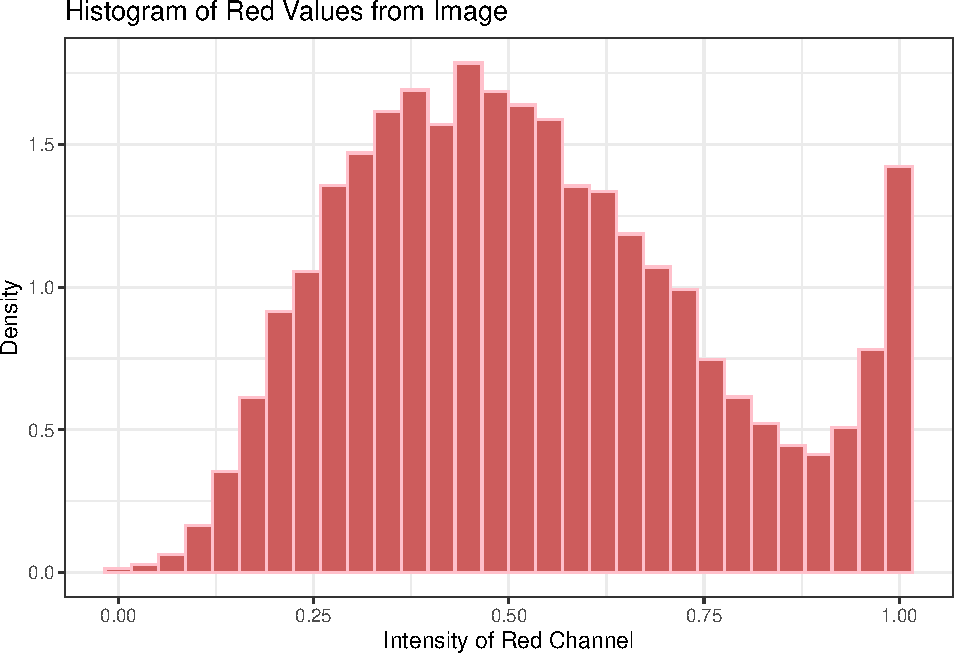
\includegraphics{03_vectors_files/figure-latex/unnamed-chunk-18-1.pdf}

this clearly shows that the Petal Width and Length have the most linear
relationship, although this may differ accross species and should be
potentially investigated with a second correlation plot or a scatter
plot.

\hypertarget{pair-wise-plot}{%
\subsubsection{Pair wise Plot}\label{pair-wise-plot}}

various pairwise scatter plots can be prepared by using the
\texttt{pairs()} function:

\begin{Shaded}
\begin{Highlighting}[]
\KeywordTok{pairs}\NormalTok{(iris\_df\_pretty)}
\end{Highlighting}
\end{Shaded}

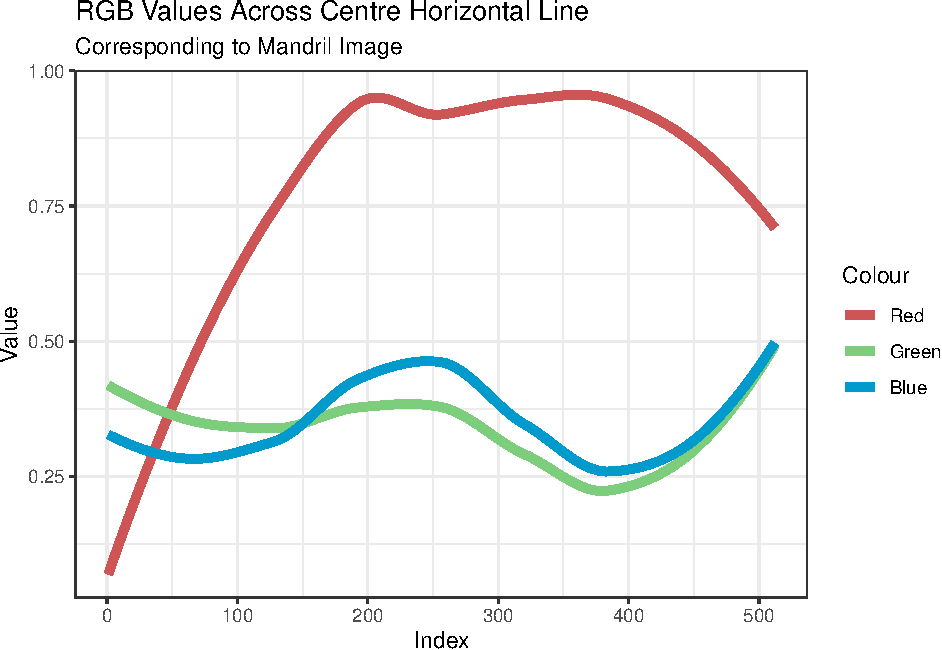
\includegraphics{03_vectors_files/figure-latex/unnamed-chunk-19-1.pdf}

If the Species Data was also to be considered that could be done by
creating a boxplot:

\begin{Shaded}
\begin{Highlighting}[]
\NormalTok{data\_cols <{-}}\StringTok{ }\KeywordTok{c}\NormalTok{(}\StringTok{"Sepal.Length"}\NormalTok{, }\StringTok{"Sepal.Width"}\NormalTok{, }\StringTok{"Petal.Length"}\NormalTok{, }\StringTok{"Petal.Width"}\NormalTok{)}
\KeywordTok{ggplot}\NormalTok{(}\DataTypeTok{data =} \KeywordTok{pivot\_longer}\NormalTok{(iris\_df, }\DataTypeTok{cols =} \KeywordTok{names}\NormalTok{(iris\_df)[}\DecValTok{2}\OperatorTok{:}\DecValTok{5}\NormalTok{]), }\KeywordTok{aes}\NormalTok{(}\DataTypeTok{x =}\NormalTok{ Species, }\DataTypeTok{fill =}\NormalTok{ name, }\DataTypeTok{y =}\NormalTok{ value)) }\OperatorTok{+}
\StringTok{  }\KeywordTok{geom\_boxplot}\NormalTok{() }\OperatorTok{+}\StringTok{ }
\StringTok{  }\KeywordTok{theme\_bw}\NormalTok{() }\OperatorTok{+}
\StringTok{  }\KeywordTok{scale\_fill\_discrete}\NormalTok{(}\DataTypeTok{labels =} \KeywordTok{c}\NormalTok{(}\StringTok{"Sepal Length"}\NormalTok{, }\StringTok{"Sepal Width"}\NormalTok{, }\StringTok{"Petal Length"}\NormalTok{, }\StringTok{"Petal Width"}\NormalTok{)) }\OperatorTok{+}
\StringTok{  }\KeywordTok{labs}\NormalTok{(}\DataTypeTok{title =} \StringTok{"Iris Measurements Across Species"}\NormalTok{)}
\end{Highlighting}
\end{Shaded}

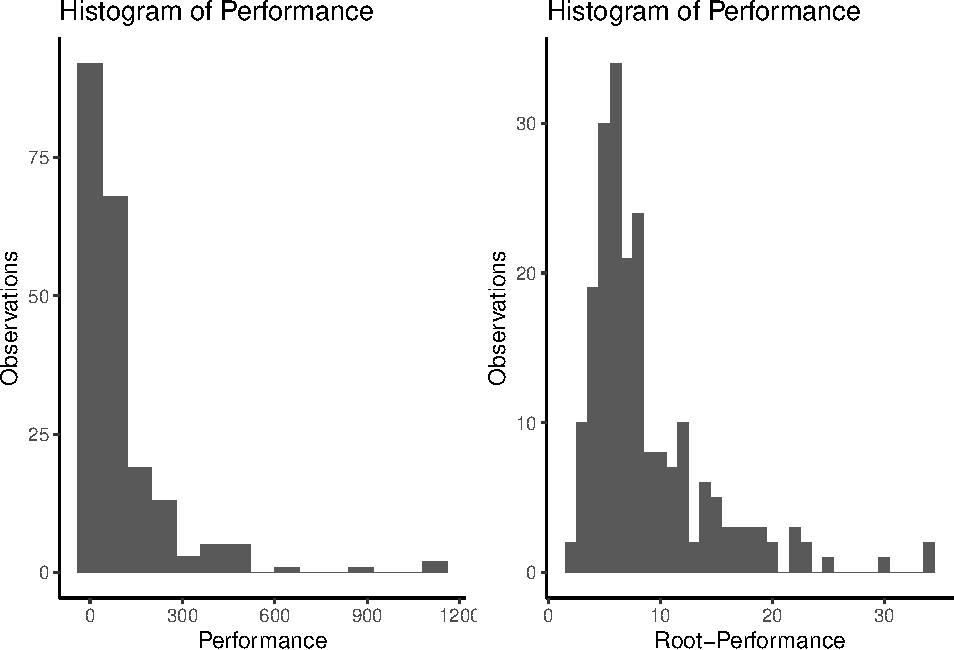
\includegraphics{03_vectors_files/figure-latex/unnamed-chunk-20-1.pdf}

\begin{Shaded}
\begin{Highlighting}[]
\CommentTok{\# names(iris\_df)}
\end{Highlighting}
\end{Shaded}

\hypertarget{create-a-linear-model}{%
\subsubsection{Create a Linear Model}\label{create-a-linear-model}}

A linear Model can be created and plotted using base packages thusly:

\begin{Shaded}
\begin{Highlighting}[]
\NormalTok{(petal\_model <{-}}\StringTok{ }\KeywordTok{lm}\NormalTok{(Petal.Length }\OperatorTok{\textasciitilde{}}\StringTok{ }\NormalTok{Petal.Width, }\DataTypeTok{data =}\NormalTok{ iris\_df))}
\end{Highlighting}
\end{Shaded}

\begin{verbatim}
## 
## Call:
## lm(formula = Petal.Length ~ Petal.Width, data = iris_df)
## 
## Coefficients:
## (Intercept)  Petal.Width  
##       1.082        2.244
\end{verbatim}

\begin{Shaded}
\begin{Highlighting}[]
\CommentTok{\# Factors are numbers under the hood so they\textquotesingle{}ll create a colour vector}
\CommentTok{\# my\_cols <{-} display.brewer.pal(3,"Accent")}
\NormalTok{my\_cols <{-}}\StringTok{ }\NormalTok{wesanderson}\OperatorTok{::}\KeywordTok{wes\_palette}\NormalTok{(}\StringTok{"Cavalcanti1"}\NormalTok{, }\DecValTok{3}\NormalTok{)}

\KeywordTok{plot}\NormalTok{(Petal.Length }\OperatorTok{\textasciitilde{}}\StringTok{ }\NormalTok{Petal.Width,}
     \DataTypeTok{data =}\NormalTok{ iris\_df, }\DataTypeTok{col =}\NormalTok{ my\_cols[iris\_df}\OperatorTok{$}\NormalTok{Species],}
     \DataTypeTok{pch =} \KeywordTok{c}\NormalTok{(}\DecValTok{15}\NormalTok{,}\DecValTok{17}\NormalTok{, }\DecValTok{19}\NormalTok{)[iris\_df}\OperatorTok{$}\NormalTok{Species],}
     \DataTypeTok{main =} \StringTok{"Linear Model of Iris Data"}\NormalTok{,}
     \DataTypeTok{xlab =} \StringTok{"Petal Width"}\NormalTok{, }
     \DataTypeTok{ylab =} \StringTok{"Petal Length"}\NormalTok{)}
\KeywordTok{abline}\NormalTok{(petal\_model, }\DataTypeTok{col =} \StringTok{"Purple"}\NormalTok{)}
\end{Highlighting}
\end{Shaded}

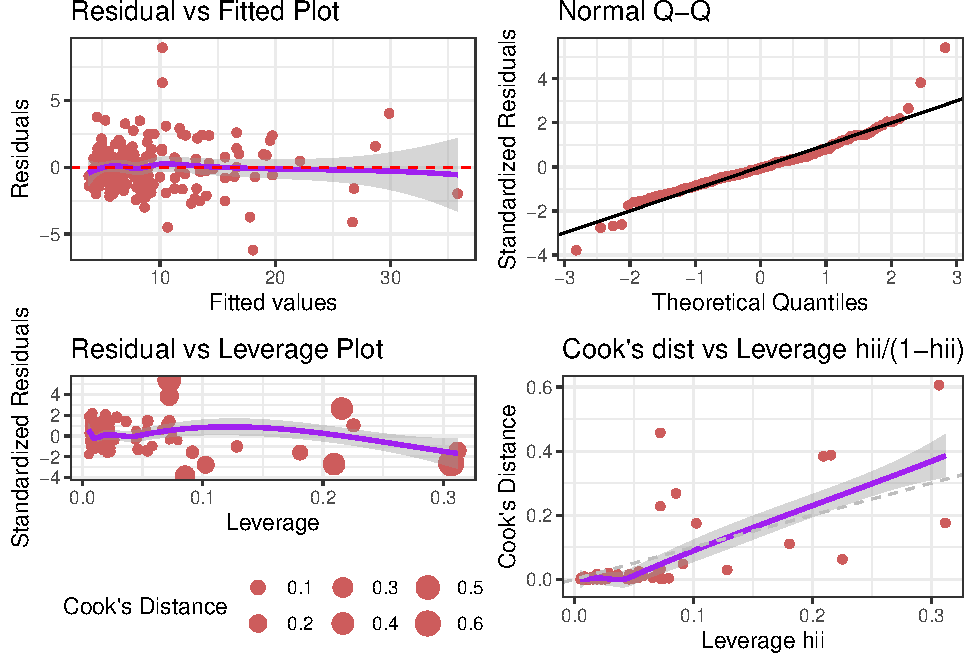
\includegraphics{03_vectors_files/figure-latex/unnamed-chunk-21-1.pdf}

This however is not very efficient, multiple linear models can be
greated and plotted using tidy data and facets in \texttt{ggplot2}:

\begin{Shaded}
\begin{Highlighting}[]
\NormalTok{iris\_tidy <{-}}\StringTok{ }\KeywordTok{pivot\_longer}\NormalTok{(iris\_df, }\DataTypeTok{cols =} \KeywordTok{names}\NormalTok{(iris\_df)[}\DecValTok{3}\OperatorTok{:}\DecValTok{5}\NormalTok{])}
\NormalTok{(iris\_tidy <{-}}\StringTok{ }\NormalTok{iris\_tidy[, }\DecValTok{{-}1}\NormalTok{])}
\end{Highlighting}
\end{Shaded}

\begin{verbatim}
## # A tibble: 354 x 4
##    Sepal.Length Species name         value
##           <dbl> <fct>   <chr>        <dbl>
##  1          5.1 setosa  Sepal.Width    3.5
##  2          5.1 setosa  Petal.Length   1.4
##  3          5.1 setosa  Petal.Width    0.2
##  4          4.9 setosa  Sepal.Width    3  
##  5          4.9 setosa  Petal.Length   1.4
##  6          4.9 setosa  Petal.Width    0.2
##  7          4.7 setosa  Sepal.Width    3.2
##  8          4.7 setosa  Petal.Length   1.3
##  9          4.7 setosa  Petal.Width    0.2
## 10          4.6 setosa  Sepal.Width    3.1
## # ... with 344 more rows
\end{verbatim}

\begin{Shaded}
\begin{Highlighting}[]
\KeywordTok{ggplot}\NormalTok{(}\DataTypeTok{data =}\NormalTok{ iris\_tidy, }\KeywordTok{aes}\NormalTok{(}\DataTypeTok{y =}\NormalTok{ Sepal.Length, }\DataTypeTok{x =}\NormalTok{ value, }\DataTypeTok{col =}\NormalTok{ name)) }\OperatorTok{+}
\StringTok{  }\KeywordTok{geom\_point}\NormalTok{() }\OperatorTok{+}\StringTok{ }
\CommentTok{\#  facet\_grid(. \textasciitilde{} name, scales = "free\_x") +}
\StringTok{  }\KeywordTok{facet\_grid}\NormalTok{(. }\OperatorTok{\textasciitilde{}}\StringTok{ }\NormalTok{name) }\OperatorTok{+}
\StringTok{  }\KeywordTok{geom\_smooth}\NormalTok{(}\DataTypeTok{method =} \StringTok{"lm"}\NormalTok{) }\OperatorTok{+}
\StringTok{  }\KeywordTok{theme\_bw}\NormalTok{() }\OperatorTok{+}
\StringTok{  }\KeywordTok{guides}\NormalTok{(}\DataTypeTok{col =} \OtherTok{FALSE}\NormalTok{) }\OperatorTok{+}
\StringTok{  }\KeywordTok{labs}\NormalTok{(}\DataTypeTok{title =} \StringTok{"Linear Models for Iris Measurements"}\NormalTok{, }\DataTypeTok{y =} \StringTok{"Sepal Length"}\NormalTok{, }\DataTypeTok{x =} \StringTok{""}\NormalTok{)}
\end{Highlighting}
\end{Shaded}

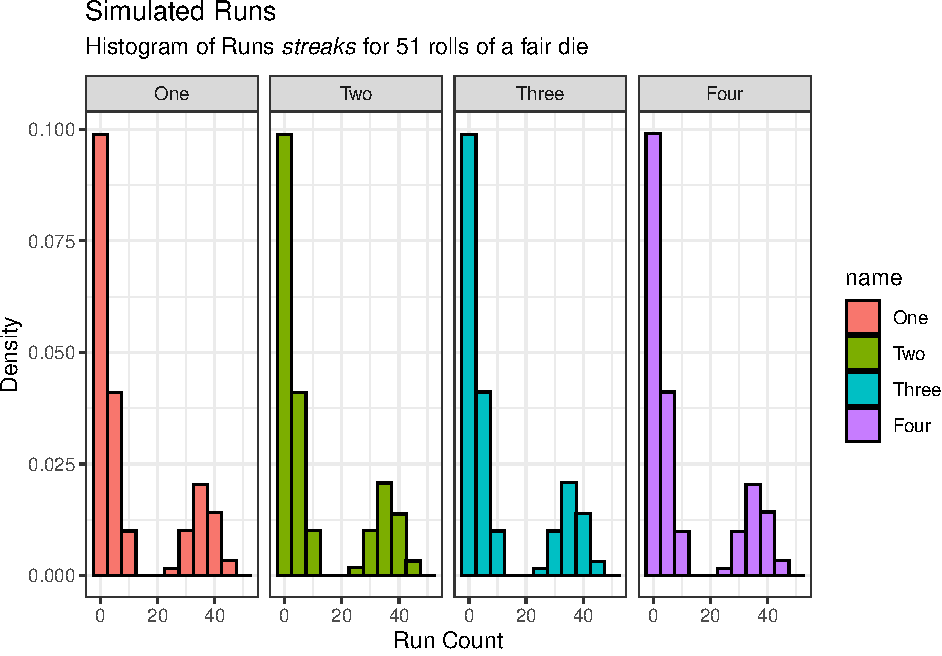
\includegraphics{03_vectors_files/figure-latex/unnamed-chunk-23-1.pdf}

\begin{Shaded}
\begin{Highlighting}[]
\NormalTok{mycols <{-}}\StringTok{ }\KeywordTok{c}\NormalTok{(}\StringTok{"darkorchid1"}\NormalTok{, }\StringTok{"limegreen"}\NormalTok{, }\StringTok{"slateblue2"}\NormalTok{, }\StringTok{"deeppink4"}\NormalTok{)}
\NormalTok{mycols <{-}}\StringTok{ }\NormalTok{mycols[}\KeywordTok{c}\NormalTok{(}\DecValTok{4}\NormalTok{,}\DecValTok{1}\NormalTok{,}\DecValTok{2}\NormalTok{,}\DecValTok{3}\NormalTok{)]}


\KeywordTok{ggplot}\NormalTok{(}\DataTypeTok{data =}\NormalTok{ iris\_tidy, }\KeywordTok{aes}\NormalTok{(}\DataTypeTok{y =}\NormalTok{ Sepal.Length, }\DataTypeTok{x =}\NormalTok{ value, }\DataTypeTok{col =}\NormalTok{ Species)) }\OperatorTok{+}
\StringTok{  }\KeywordTok{geom\_point}\NormalTok{() }\OperatorTok{+}\StringTok{ }
\CommentTok{\#  facet\_grid(. \textasciitilde{} name, scales = "free\_x") +}
\StringTok{  }\KeywordTok{facet\_grid}\NormalTok{(. }\OperatorTok{\textasciitilde{}}\StringTok{ }\NormalTok{name) }\OperatorTok{+}
\StringTok{  }\KeywordTok{stat\_smooth}\NormalTok{(}\DataTypeTok{method =} \StringTok{"lm"}\NormalTok{, }\DataTypeTok{se =} \OtherTok{FALSE}\NormalTok{) }\OperatorTok{+}
\StringTok{  }\KeywordTok{theme\_bw}\NormalTok{() }\OperatorTok{+}
\StringTok{  }\KeywordTok{labs}\NormalTok{(}\DataTypeTok{title =} \StringTok{"Linear Models for Iris Measurements"}\NormalTok{, }\DataTypeTok{y =} \StringTok{"Sepal Length"}\NormalTok{, }\DataTypeTok{x =} \StringTok{""}\NormalTok{) }\OperatorTok{+}
\CommentTok{\#  scale\_color\_discrete(c("Setosa", "Versicolor", "Virginica")) +}
\StringTok{  }\KeywordTok{stat\_smooth}\NormalTok{(}\KeywordTok{aes}\NormalTok{(}\DataTypeTok{group =} \DecValTok{1}\NormalTok{, }\DataTypeTok{col =} \StringTok{"All"}\NormalTok{), }\DataTypeTok{method =} \StringTok{"lm"}\NormalTok{, }\DataTypeTok{se =} \OtherTok{FALSE}\NormalTok{) }\OperatorTok{+}
\StringTok{  }\KeywordTok{scale\_color\_manual}\NormalTok{(}\DataTypeTok{labels=} \KeywordTok{c}\NormalTok{(}\StringTok{"All"}\NormalTok{, }\StringTok{"Setosa"}\NormalTok{, }\StringTok{"Versicolor"}\NormalTok{, }\StringTok{"Virginica"}\NormalTok{),}
                     \DataTypeTok{values =}\NormalTok{ mycols)}
\end{Highlighting}
\end{Shaded}

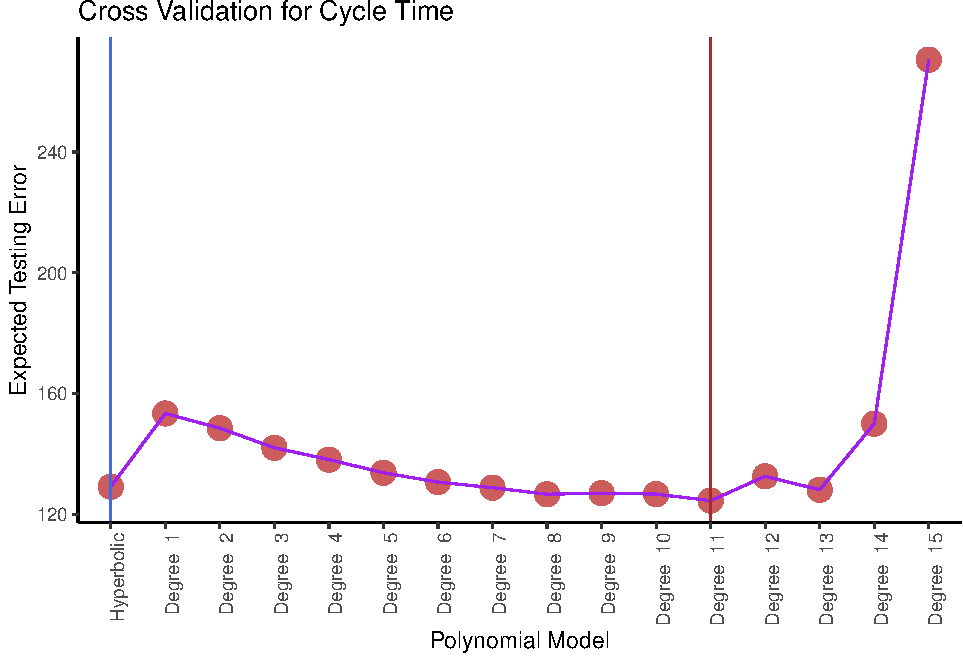
\includegraphics{03_vectors_files/figure-latex/unnamed-chunk-24-1.pdf}

\end{document}
